\documentclass[dtu]{dtuarticle}
\usepackage{parskip} % use enters instead of indents

%\newcommand{\todo}[1]{\color{red}[TODO: #1]\color{black}}
\newcommand*\chem[1]{\ensuremath{\mathrm{#1}}}
\usepackage{amsmath}
\usepackage{bm}
\usepackage{siunitx}
\sisetup{
    per-mode=fraction,
    detect-weight = true,
    detect-family = true,
    separate-uncertainty=true,
    output-decimal-marker={.}
}

\usepackage{subcaption}
\usepackage{booktabs}
\usepackage{listings}
\usepackage{graphicx}
\usepackage{url}
\usepackage{listings}
\usepackage{xcolor}
\usepackage{float}

\lstdefinestyle{sql}{
    language=SQL,
    basicstyle=\ttfamily\small,
    keywordstyle=\color{blue},
    commentstyle=\color{gray},
    stringstyle=\color{orange},
    showstringspaces=false,
    breaklines=true
}


\title{02327 Introductory Databases and Database Programming Mandatory Project}
\subtitle{Cykelparadis DB: Design, Implem., SQL}
\author{Group 08}
\course{02327 Introductory Databases and Database Programming}
\address{
    DTU Compute \\
    Fall 2025
}
\date{\today}

\begin{document}

\maketitle

% --------------------------------------------------------
% GROUP INFORMATION
% --------------------------------------------------------
\begin{table}[h!]
\renewcommand{\arraystretch}{1.2}
\centering
\begin{subtable}{\textwidth}
    \centering
    \begin{tabular}{l | l}
        \textbf{Name} & \textbf{Student number} \\ \hline\hline
        Sam Baghban Golpasand & s256281 \\ \hline
        Diego Armando Mijares Ledezma & s251777 \\ \hline
        Ulaş Sertan Kemec & s252236 \\ \hline
        Albert Ronnenberg Kirk & s256201 \\ \hline
        Setara Hussaini & s255904
    \end{tabular}
    \caption{Group members.}
\end{subtable}
\\[0.25cm]
\begin{subtable}{\textwidth}
    \centering
    \begin{tabular}{l | *{5}{|r}}
        \textbf{Task} & \textbf{Sam} & \textbf{Diego} & \textbf{Ulaş} & \textbf{Albert} & \textbf{Setara} \\ \hline\hline
        Conceptual Design & 20\% & 20\% & 20\% & 20\% & 20\% \\ \hline
        Logical Design & 20\% & 20\% & 20\% & 20\% & 20\% \\ \hline
        Implementation & 10\% & 10\% & 30\% & 40\% & 10\% \\ \hline
        Database Instance & 10\% & 10\% & 20\% & 30\% & 30\% \\ \hline
        SQL Table Modifications & 20\% & 30\% & 10\% & 10\% & 30\% \\ \hline
        SQL Queries & 20\% & 30\% & 30\% & 10\% & 10\% \\ \hline
        SQL Programming & 40\% & 20\% & 10\% & 10\% & 20\% \\ \hline
        \textbf{Average of all above} & \textbf{20\%} & \textbf{20\%} & \textbf{20\%} & \textbf{20\%} & \textbf{20\%} \\ \hline

    \end{tabular}
    \caption{Contributions \& responsibilities table.}
\end{subtable}
\caption{Group information \& work distribution.}
\end{table}

\tableofcontents
\newpage

\section{Introduction}

The \textbf{purpose} of this project is to design, implement, and manipulate a relational database for a bicycle repair shop named Cykelparadis. The database aims to efficiently store information about customers, bicycles, parts, manufacturers, and repair jobs, while ensuring data consistency, integrity, and ease of retrieval.

The \textbf{objective} is twofold:  
1. To create a robust database schema that accurately represents the real-world entities and relationships involved in the repair shop operations, ensuring adherence to database design principles such as normalization and constraint enforcement.  
2. To demonstrate the practical usage of SQL through table creation, data manipulation, querying, and programming constructs such as functions, procedures, and triggers to automate and validate business rules.

By completing this project, we showcase the end-to-end process of database development: from conceptual modeling to logical design, implementation, and verification through queries and procedural logic.

% ========================================================
\section{Conceptual design}
% ========================================================

The conceptual design provides a high-level representation of the system using the adapted UML notation presented in the textbook \cite{silberschatz2019db}. It captures the main entity sets, their attributes, and the relationships between them before any translation into relational structures.

\begin{figure}[h!]
    \centering
    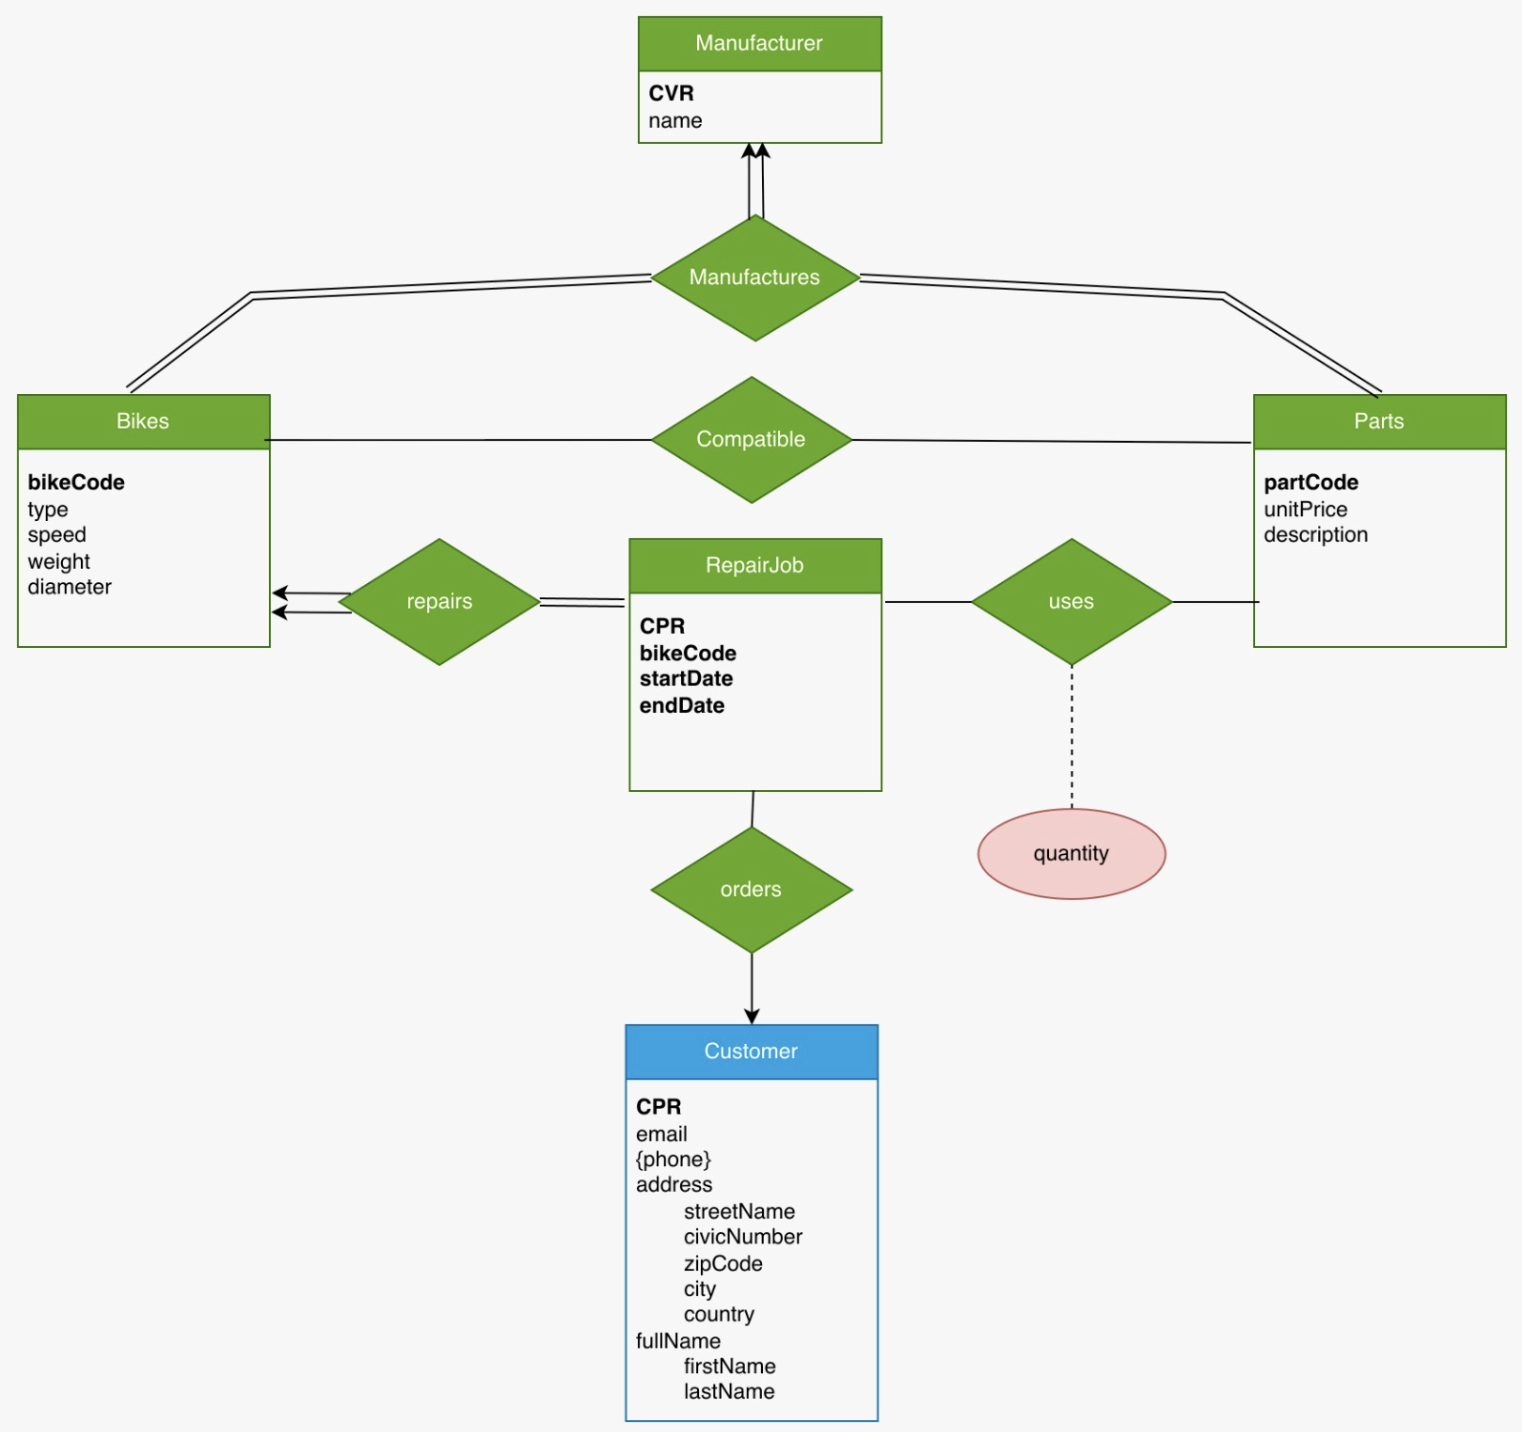
\includegraphics[width=0.85\textwidth]{figures/er_diagram.png}
    \caption{Entity-relationship diagram for the Cykelparadis database.}
    \label{fig:er}
\end{figure}

\subsection*{Entities and relationships explained along design choices}

In our model, \textbf{primary keys} are written in bold, and attributes of relationship sets are represented with oval shapes in the ER diagram. The rhomboids (diamonds) represent relationship sets.

\paragraph{Manufacturer}
For the entity set \textit{Manufacturer}, we initially considered using only \textit{name} as the primary key. However, this was rejected because (i) two manufacturers may share the same name, and (ii) manufacturers may change their name over time. Therefore, we use the CVR number as the primary key, as it provides a unique and persistent identifier for each manufacturer.

\paragraph{Bikes}
The entity set \textit{Bikes} includes the attributes \textbf{bikeCode} (primary key), \textit{type}, \textit{speeds}, \textit{weight}, and \textit{diameter}. The attribute \textit{bikeCode} is interpreted as the vehicle identification number (stelnummer), which is inherently unique for each bike, making it a sufficient primary key.

\paragraph{Parts}
The entity set \textit{Parts} contains the attributes \textbf{partCode} (primary key), \textit{unitPrice}, and \textit{description}.

\paragraph{Manufactures (ternary relationship)}
The entity sets \textit{Manufacturer}, \textit{Parts}, and \textit{Bikes} participate in a ternary relationship set \textit{manufactures}. Each of the three entity sets has total participation in this relationship. We do not consider cases where a bike or part lacks a manufacturer, nor do we store manufacturers that have not yet produced any of the bikes or parts in our database.

The relationship is one-to-many from \textit{Manufacturer} to both \textit{Bikes} and \textit{Parts}: a manufacturer may produce many bikes and parts, but each bike or part is assumed to be produced by exactly one manufacturer.

\paragraph{Compatible}
\textit{Bikes} and \textit{Parts} share a many-to-many relationship set \textit{Compatible}, which stores which bikes are compatible with which parts. Because some bikes may have no compatible parts and some parts may have no compatible bikes, neither entity set has total participation in this relationship.

\paragraph{Customer}
The entity set \textit{Customer} includes the attributes \textbf{CPR} (primary key), \textit{email}, \textit{phoneNumber}, \textit{address} (consisting of \textit{street}, \textit{civicNumber}, \textit{city}, \textit{zipCode}, \textit{country}), and \textit{name} (consisting of \textit{firstName} and \textit{lastName}).

\paragraph{RepairJobs}
The entity set \textit{RepairJobs} includes the attributes \textit{startDate} and \textit{endDate}. Together with \textit{CPR} (from \textit{Customer}) and \textit{bikeCode} (from \textit{Bikes}), these form a composite primary key for \textit{RepairJobs}.

\paragraph{Repairs}
\textit{Bikes} participates in a one-to-many relationship set \textit{repairs} with \textit{RepairJobs}: A bike may have multiple repair jobs, but each repair job pertains to exactly one bike.

\paragraph{Uses}
\textit{RepairJobs} also participates in a many-to-many relationship set \textit{uses} with \textit{Parts}. A part may be used in multiple repair jobs, and a repair job may require multiple parts. Because we need to record the \textit{quantity} of parts used per repair job, \textit{quantity} is included as an attribute of the relationship set \textit{uses}.

\paragraph{Orders}
Finally, \textit{Customer} shares a one-to-many relationship set \textit{orders} with \textit{RepairJobs}: A customer may request multiple repair jobs, but each repair job is associated with exactly one customer. A customer may solicit multiple repairs, but a repair is assumed to have been solicited by exactly one customer.

% ========================================================
\section{Logical Design}
% ========================================================

The conceptual ER model is translated into a logical relational schema, where entities, relationships, and constraints are represented using tables, primary keys, foreign keys, and normalization principles. This section presents the resulting relational schema and its structure.

\subsection*{Database Schema Diagram}

Again, \textbf{primary keys} are bold, with the addition of underlined \underline{foreign keys}. 

\begin{figure}[h!]
    \centering
    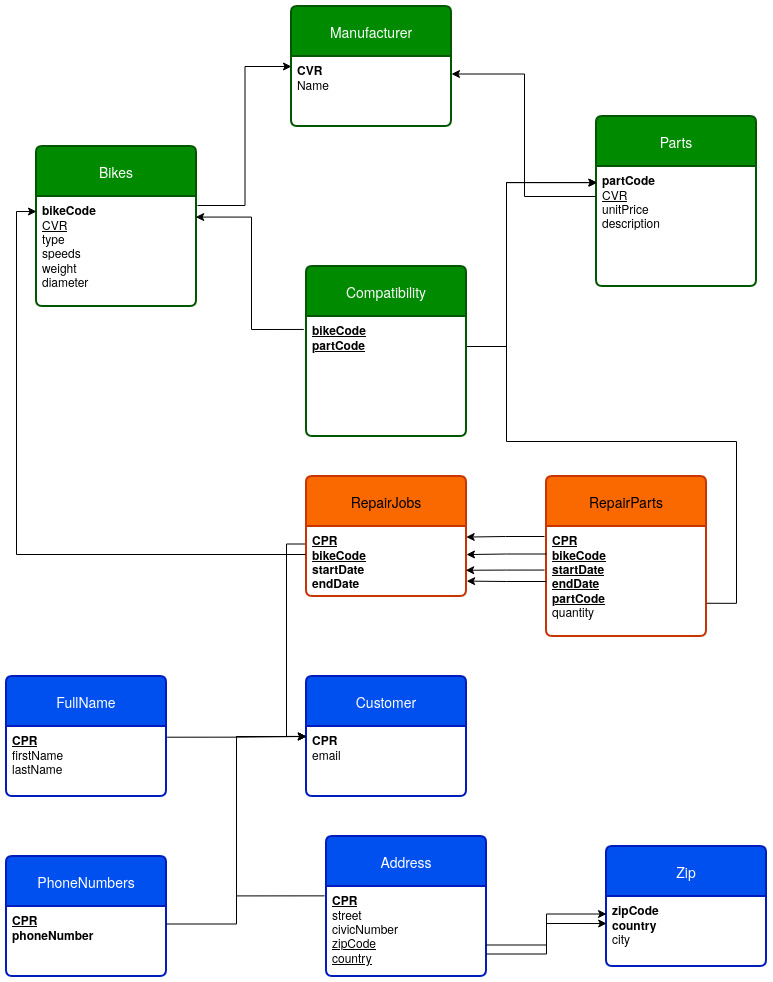
\includegraphics[width=0.85\textwidth]{figures/schema_diagram_new.png}
    \caption{Database schema diagram (logical design).}
    \label{fig:schema}
\end{figure}

\subsection*{Discussion of Design Choices}

\paragraph{Normalization}
Our logical schema has been designed to satisfy Third Normal Form (3NF). All attributes depend solely on the primary key of their respective tables, and no transitive dependencies remain.

For the \textit{Customer} entity, we avoid storing composite or multi-valued attributes inside a single table. Thus, \textit{phoneNumber} is stored in its own table, using \underline{CPR} together with the phone number as the primary key, since a customer may have multiple phone numbers. Likewise, \textit{firstName} and \textit{lastName} are stored in a separate table to ensure that both attributes remain fully functionally dependent on \underline{CPR}. 

The attribute \textit{address} is decomposed to eliminate transitive dependencies: since \textit{zipCode} and \textit{country} functionally determine \textit{city}, these attributes are placed in a separate \textit{Zip} table. The \textit{Address} table references \textit{zipCode} and \textit{country} and uses \underline{CPR} as its primary key. This decomposition ensures that no non-key attribute depends transitively on the primary key of \textit{Customer}.

For the entity sets \textit{Bikes} and \textit{Parts}, no normalization beyond ensuring atomic attributes is required, since their primary keys (\textbf{bikeCode} and \textbf{partCode}) fully determine all remaining attributes.

\paragraph{Foreign Keys and Relationship Implementation}
Each relationship in the conceptual model has been mapped to the relational schema using standard ER-to-relational mapping rules.

The ternary relationship \textit{Manufactures} cannot be represented directly as a table without unnecessarily storing redundant combinations. Instead, we use foreign keys in the existing tables to establish the relationship: both \textit{Bike} and \textit{Part} contain \underline{CVR} as a foreign key referencing \textit{Manufacturer}. Since each bike and part is uniquely identified by its respective code, the foreign key does not form part of the primary key.

The many-to-many relationship \textit{Compatible} between \textit{Bikes} and \textit{Parts} is implemented as a bridge table, \textit{Compatible}, whose composite primary key consists of \underline{bikeCode} and \underline{partCode}. This table captures which parts are compatible with which bikes without introducing redundancy.

The entity \textit{RepairJobs} becomes its own table with attributes \textit{startDate}, \textit{endDate}, \textit{bikeCode}, and \underline{\textbf{CPR}}. Together, these attributes form a composite primary key, ensuring that two repair jobs involving the same customer and the same bike cannot overlap in the same time interval. 

The many-to-many relationship \textit{uses} between \textit{RepairJobs} and \textit{Parts} is implemented as the table \textit{RepairParts}, with primary key (\underline{\textbf{bikeCode}}, \underline{\textbf{CPR}}, \underline{\textbf{startDate}}, \underline{\textbf{endDate}}, \underline{\textbf{partCode}}) and with the relationship attribute \textit{quantity} included.


\paragraph{Partial vs.\ Full Participation}
The mapping also respects partial and full participation from the conceptual model:

\begin{itemize}
    \item \textit{Manufactures} is in full participation for all three entity sets: every stored \textit{Bike} and \textit{Part} must reference a \textit{Manufacturer}, and we do not store manufacturers without produced items.
    \item \textit{Compatible} is in partial participation for both \textit{Bikes} and \textit{Parts}: some bikes may have no compatible parts, and some parts may not be compatible with any bike.
    \item The relationship \textit{repairs} is in full participation for \textit{RepairJobs}, since each repair job must refer to one bike, and is likewise mandatory for \textit{Bikes}, since a bike would not be recorded in the database without having at least one repair.
    \item The relationship \textit{orders} is in full participation for \textit{RepairJobs}, as each repair job is requested by exactly one customer, but partial for \textit{Customer}, since a customer may not have submitted any repair orders.
\end{itemize}

These choices ensure that the logical model enforces the same participation constraints as the conceptual ER model.

\paragraph{Excluded Derived Attributes}
Certain attributes that can be calculated from existing data are intentionally excluded from the schema. For example, we do not store:
\begin{itemize}
    \item the total cost of a repair job (derivable from \textit{unitPrice} and \textit{quantity}),
    \item the number of parts used in a repair (derivable from the \textit{RepairParts} table),
\end{itemize}
as storing derived values would introduce redundancy and potential inconsistency. By excluding derived attributes, we maintain normalization and data integrity.

Overall, with our design choices we looked to prioritize normalization, integrity constraints, foreign key structure, and representational clarity, whilst remaining consistent with the requirements of the project.

% ========================================================

\section{Implementation}
% ========================================================

The implementation phase consists of translating the logical design into an operational database using MariaDB. This involves creating the database schema, defining tables, specifying primary and foreign key constraints, and ensuring that all relationships and integrity constraints from the logical model are correctly enforced. The following subsection presents the SQL statements used to create the database and its associated tables, reflecting the structure and constraints established during the design phase.

\subsection*{Database Creation}
% --------------------------------------------------------

Creation of the database. It will be used to be able to create tables in it.

\begin{figure}[H]
    \centering
    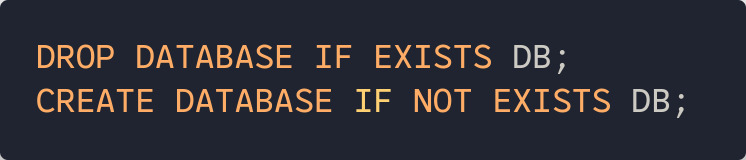
\includegraphics[width=0.9\linewidth]{figures/db_creation.png}
    \caption{SQL code for creating the database.}
    \label{fig:db_creation}
\end{figure}

% --------------------------------------------------------
\subsection*{Manufacturer Table}

The \texttt{Manufacturer} table holds a CVR number (stored as a string), unique to each manufacturer, and the name of the manufacturer. Since the CVR number is unique, it is selected as the primary key, representing the smallest subset of the candidate keys. The CVR attribute must not be \texttt{NULL} to satisfy primary key requirements.

\begin{figure}[H]
    \centering
    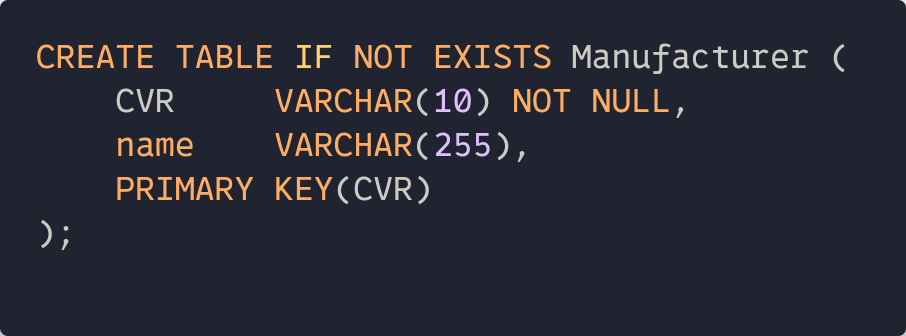
\includegraphics[width=0.9\linewidth]{figures/manufacturer_table.png}
    \caption{SQL code for creating the \texttt{Manufacturer} table.}
    \label{fig:manufacturer_table}
\end{figure}

% --------------------------------------------------------
\subsection*{Bike Table}

The \texttt{Bikes} table holds a \texttt{bikeCode} string of length 10, which acts as the primary key. The table also contains attributes such as \texttt{type}, \texttt{CVR}, \texttt{speed}, and \texttt{wheelDiameter}. The \texttt{CVR} attribute is a foreign key referencing the \texttt{Manufacturer} table.

\begin{figure}[H]
    \centering
    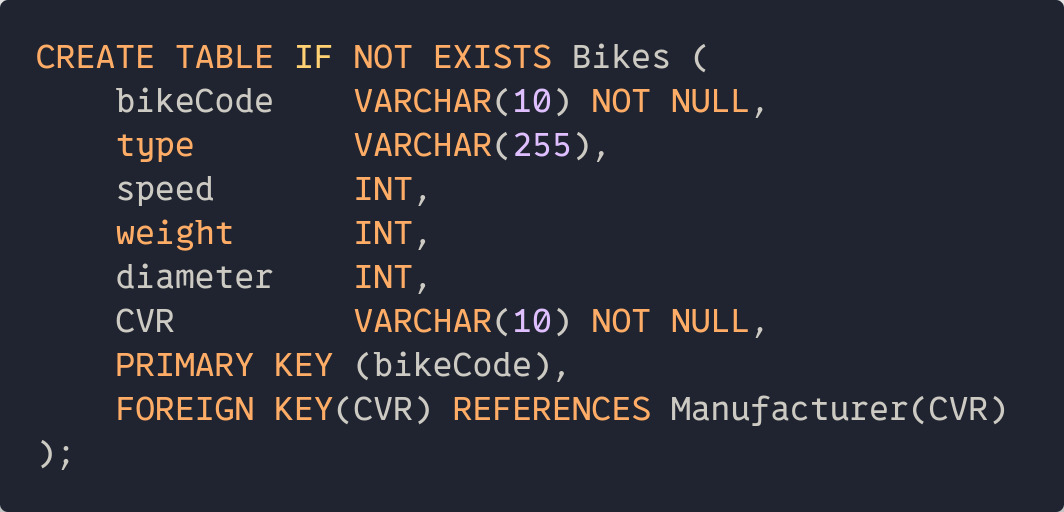
\includegraphics[width=0.9\linewidth]{figures/bike_table.png}
    \caption{SQL code for creating the \texttt{Bikes} table.}
    \label{fig:bike_table}
\end{figure}

% --------------------------------------------------------
\subsection*{Parts Table}

The \texttt{Parts} table stores a \texttt{partCode} string (length 10) as the primary key. It includes the unit price, description, and CVR number. The CVR attribute is a foreign key referencing the manufacturer of the part. Since every part must have a part code and manufacturer, both are declared \texttt{NOT NULL} to prevent inconsistent insertions.

\begin{figure}[H]
    \centering
    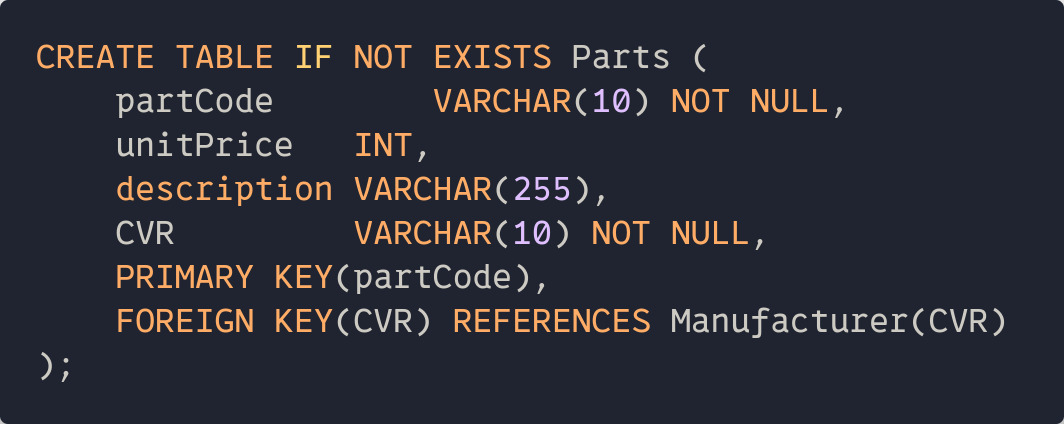
\includegraphics[width=0.9\linewidth]{figures/parts_table.png}
    \caption{SQL code for creating the \texttt{Parts} table.}
    \label{fig:parts_table}
\end{figure}

% --------------------------------------------------------
\subsection*{Compatibility Table}

The \texttt{Compatibility} table represents the relationship between bikes and parts. It stores pairs of compatible bike codes and part codes. Together, they form a composite primary key, while also serving as foreign keys referencing their respective tables. Both attributes are required to be \texttt{NOT NULL}.

\begin{figure}[H]
    \centering
    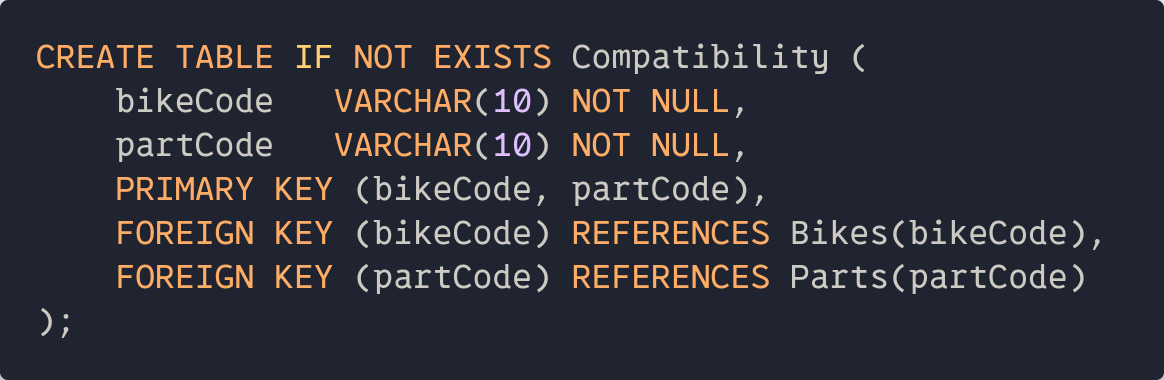
\includegraphics[width=0.9\linewidth]{figures/compatibility_table.png}
    \caption{SQL code for creating the \texttt{Compatibility} table.}
    \label{fig:compatibility_table}
\end{figure}

% --------------------------------------------------------
\subsection*{Customer Table}

The \texttt{Customer} table stores the customer's CPR number and email address. The CPR number is used as the primary key due to its uniqueness. As with all primary keys, the attribute is declared \texttt{NOT NULL} to guarantee accurate database behavior.

\begin{figure}[H]
    \centering
    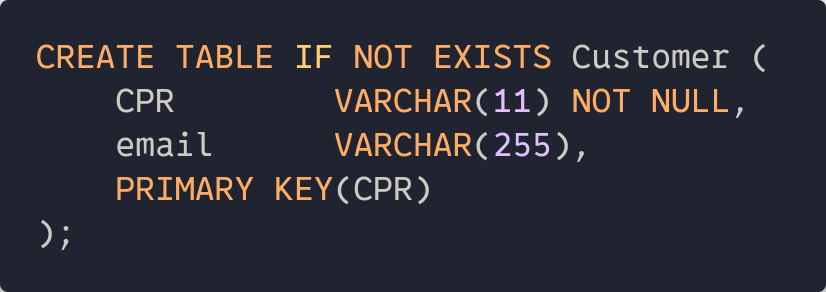
\includegraphics[width=0.9\linewidth]{figures/customer_table.png}
    \caption{SQL code for creating the \texttt{Customer} table.}
    \label{fig:customer_table}
\end{figure}

% --------------------------------------------------------
\subsection*{RepairJob Table}

The \texttt{RepairJob} table stores all information related to a repair. Its primary key consists of CPR, bike code, start date, and end date. The date attributes are essential because a customer can have multiple repairs, and the combination of dates differentiates them.

\begin{figure}[H]
    \centering
    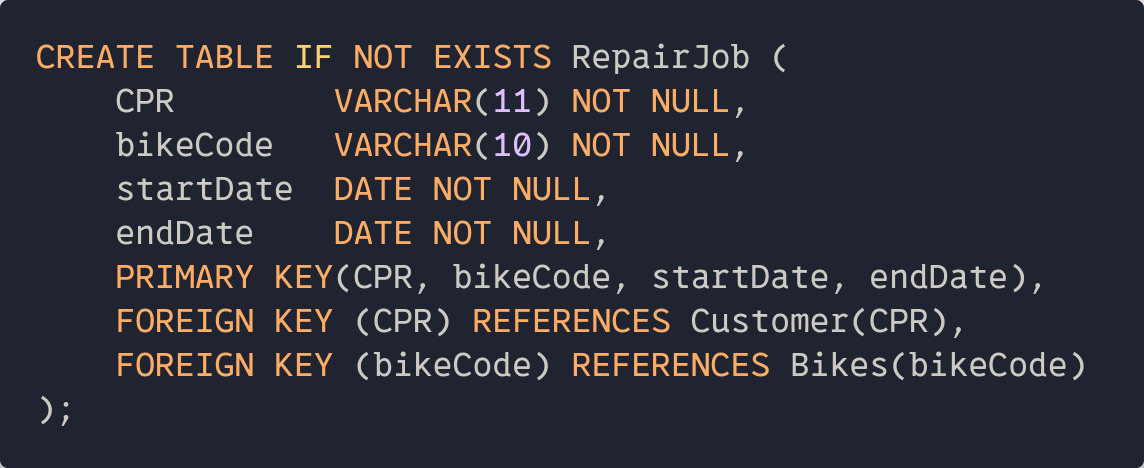
\includegraphics[width=0.9\linewidth]{figures/repairjob_table.png}
    \caption{SQL code for creating the \texttt{RepairJob} table.}
    \label{fig:repairjob_table}
\end{figure}

% --------------------------------------------------------
\subsection*{RepairParts Table}

The \texttt{RepairParts} table captures which parts are used in a particular repair job. Its primary keys are CPR, bike code, part code, start date, and end date. All keys except part code are foreign keys referencing the \texttt{RepairJob} table. The table also includes a \texttt{quantity} attribute indicating the number of units used. Deleting a row from \texttt{RepairJob} cascades the deletion to \texttt{RepairParts}, since it is a subset relationship.

\begin{figure}[H]
    \centering
    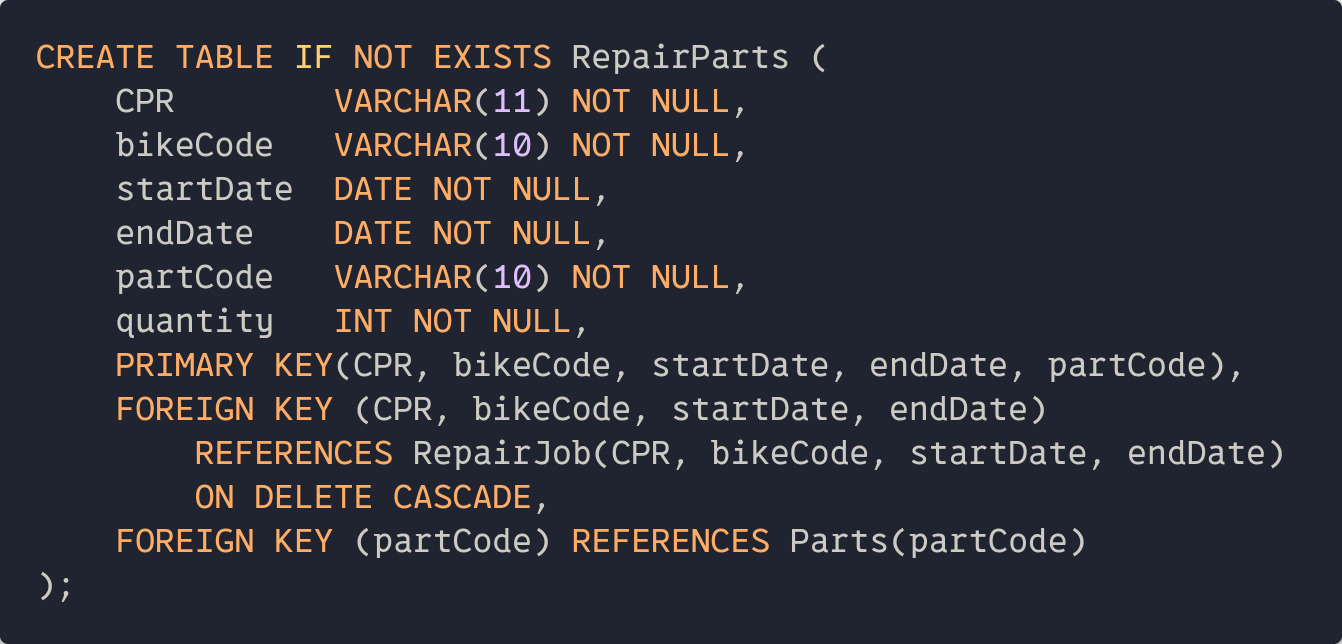
\includegraphics[width=0.9\linewidth]{figures/repairparts_table.png}
    \caption{SQL code for creating the \texttt{RepairParts} table.}
    \label{fig:repairparts_table}
\end{figure}

% --------------------------------------------------------
\subsection*{FullName Table}

The \texttt{FullName} table stores the first and last name associated with a given CPR number. CPR is both the primary key and a foreign key referencing the \texttt{Customer} table.

\begin{figure}[H]
    \centering
    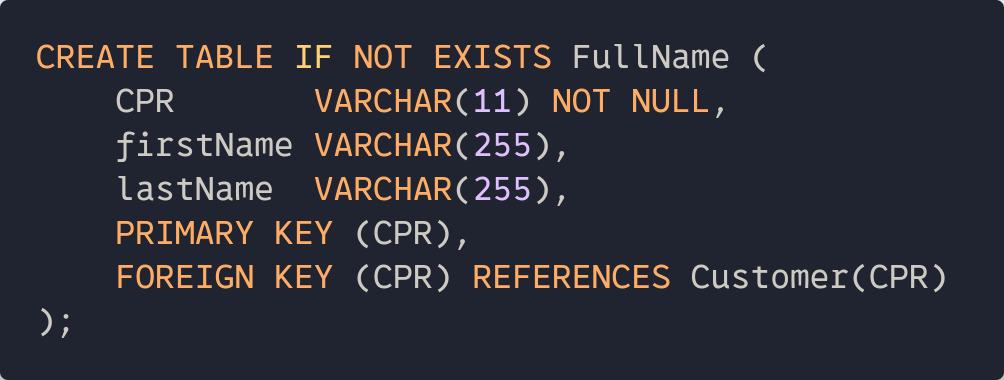
\includegraphics[width=0.9\linewidth]{figures/fullname_table.png}
    \caption{SQL code for creating the \texttt{FullName} table.}
    \label{fig:fullname_table}
\end{figure}

% --------------------------------------------------------
\subsection*{PhoneNumber Table}

The \texttt{PhoneNumber} table contains CPR and a phone number, with CPR being the primary key. CPR is also a foreign key referencing the \texttt{Customer} table.

\begin{figure}[H]
    \centering
    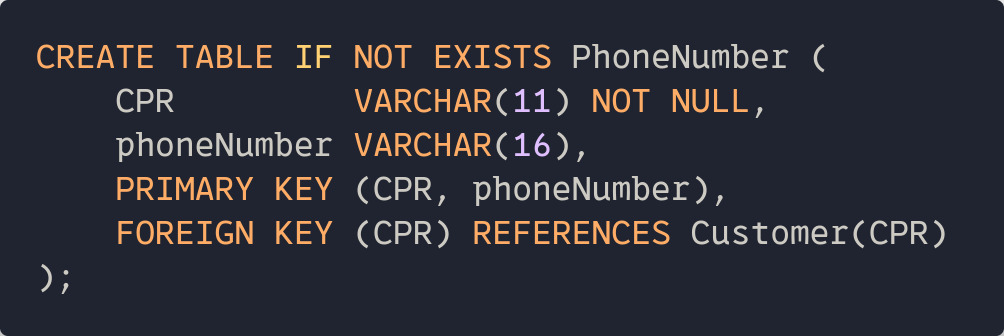
\includegraphics[width=0.9\linewidth]{figures/phonenumber_table.png}
    \caption{SQL code for creating the \texttt{PhoneNumber} table.}
    \label{fig:phonenumber_table}
\end{figure}

% --------------------------------------------------------
\subsection*{Zip Table}

The \texttt{Zip} table was generated during the normalization process. It stores the zip code, country, and city. The combination of zip code and country forms its composite primary key, since a zip code is dependent on the country.

\begin{figure}[H]
    \centering
    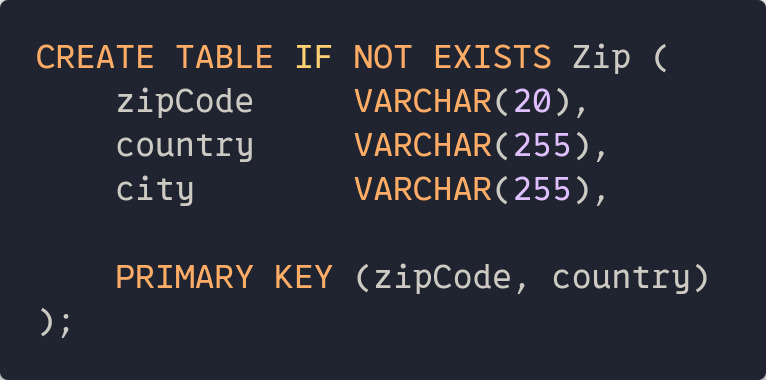
\includegraphics[width=0.9\linewidth]{figures/zipinfo_table_new.png}
    \caption{SQL code for creating the \texttt{Zip} table.}
    \label{fig:zipinfo_table}
\end{figure}

% --------------------------------------------------------
\subsection*{Address Table}

The \texttt{Address} table contains a person's address and is uniquely identified by CPR. It stores street name, civic number, zip code, and country. The latter two are foreign keys referencing the \texttt{Zip} table.

\begin{figure}[H]
    \centering
    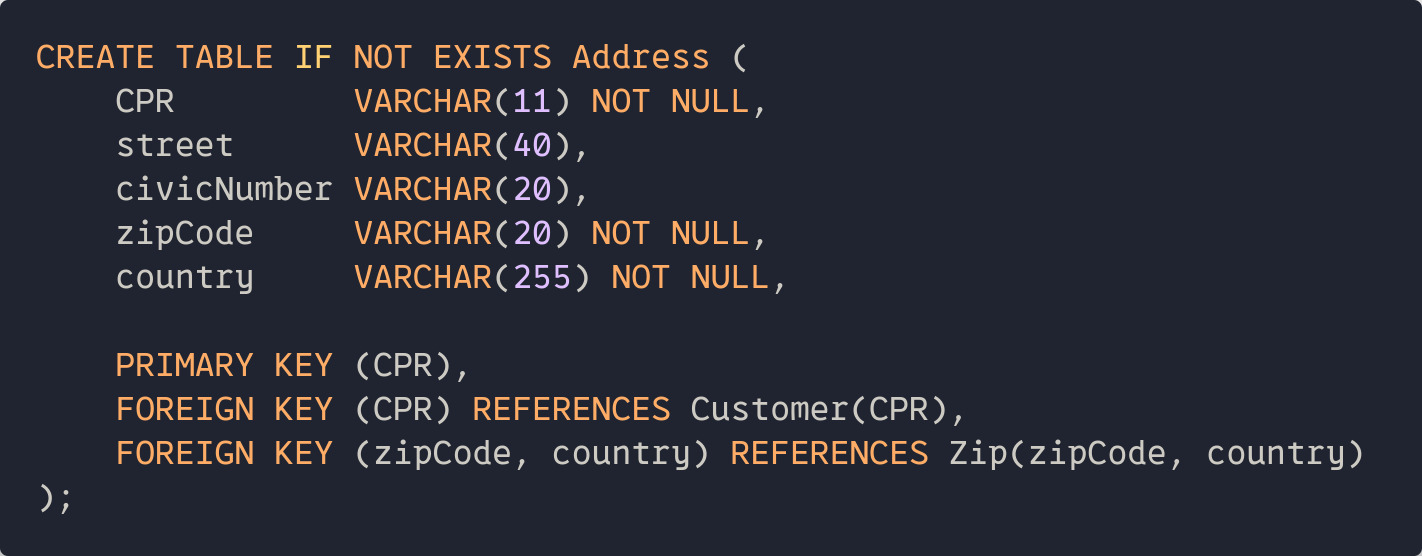
\includegraphics[width=0.9\linewidth]{figures/address_table_1.png}
    \caption{SQL code for creating the \texttt{Address} table.}
    \label{fig:address_table_1}
\end{figure}


% ========================================================
\section{Database Instance}
% ========================================================

This section presents the populated instance of the database after inserting representative sample data into all tables. 
Once the data was added, each table and view was inspected using \texttt{SELECT *} queries to verify that the database 
was correctly populated and that all constraints, relationships, and dependencies functioned as intended.

To provide a clear overview of the final state of the database, two summary figures are included.  
Figure~\ref{fig:instance1} shows the populated core operational tables: \texttt{RepairParts}, \texttt{RepairJob}, 
\texttt{Compatibility}, \texttt{Parts}, \texttt{Bikes}, and \texttt{Manufacturers}.  
Figure~\ref{fig:instance2} displays the populated supporting tables: \texttt{PhoneNumber}, \texttt{Customer}, 
\texttt{FullName}, \texttt{Address}, and \texttt{Zip}.

The following subsections include the detailed outputs of the \texttt{SELECT *} queries for each table and view. 
These results provide a complete overview of the final database instance and confirm that the schema behaves correctly 
with real data.

\begin{figure}[h!]
    \centering
    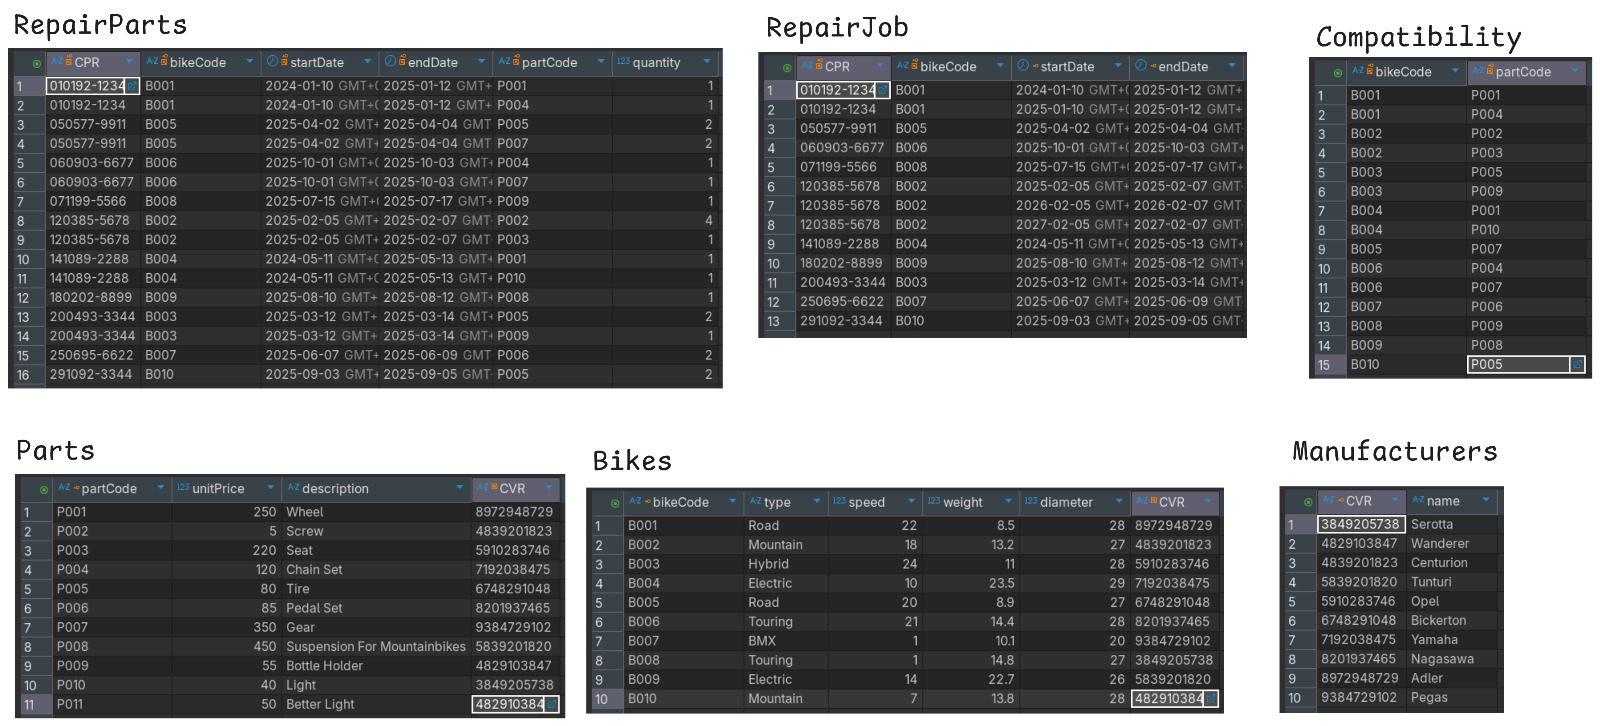
\includegraphics[width=\textwidth]{figures/instance_core_tables_placeholder.png}
    \caption{Database instance overview: RepairParts, RepairJob, Compatibility, Parts, Bikes, Manufacturers}
    \label{fig:instance1}
\end{figure}

\begin{figure}[h!]
    \centering
    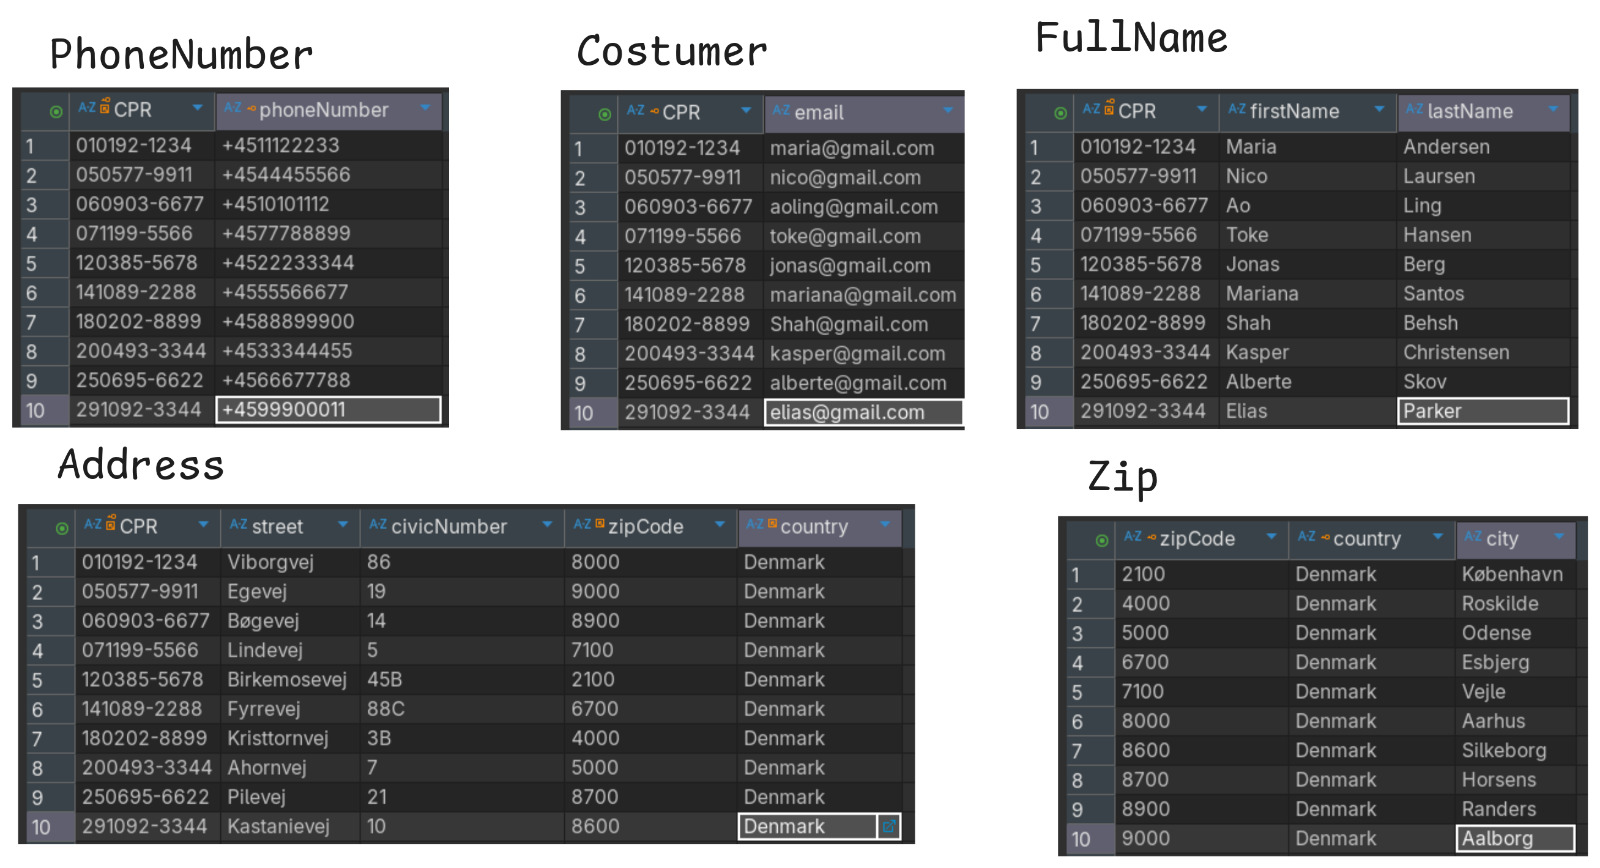
\includegraphics[width=\textwidth]{figures/instance_secondary_tables_placeholder.png}
    \caption{Database instance overview: PhoneNumber, Customer, FullName, Address, Zip}
    \label{fig:instance2}
\end{figure}


% ========================================================
\section{SQL Table Modifications}
% ========================================================

In this section, we demonstrate how data in our relational database can be modified using the core SQL data manipulation commands: \texttt{INSERT}, \texttt{UPDATE}, and \texttt{DELETE}. These operations allow us to dynamically add new entries, change existing information, and remove outdated or invalid data from the database.

According to the project requirements, we present concrete examples of:
\begin{itemize}
    \item inserting new rows into tables using \texttt{INSERT},
    \item updating existing rows using \texttt{UPDATE}, and
    \item removing rows using \texttt{DELETE}.
\end{itemize}

Only the SQL statements related to the demonstrated examples are shown here.  
Additional table modifications can be found in the full second SQL script included in the appendix.

\subsection{INSERT Examples}

\subsubsection*{Inserting a New Bike}

The following SQL statement inserts a new bicycle into the \texttt{Bikes} table.  
This example corresponds to the before-and-after screenshots shown in Figures~\ref{fig:bike-before} and \ref{fig:bike-after}.

\begin{lstlisting}[style=sql, caption={Insert a new bike into the Bikes table}, label={lst:insert-bike}]
INSERT INTO Bikes
VALUES ('B011', 'Touring', 28, 29, 25, '8972948729');
\end{lstlisting}

\begin{figure}[H]
    \centering
    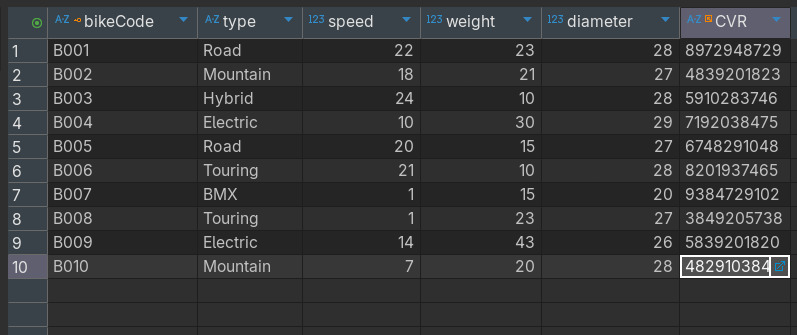
\includegraphics[width=0.9\linewidth]{figures/bikes_before_insert.png}
    \caption{Bikes table before inserting bicycle B011}
    \label{fig:bike-before}
\end{figure}

\begin{figure}[H]
    \centering
    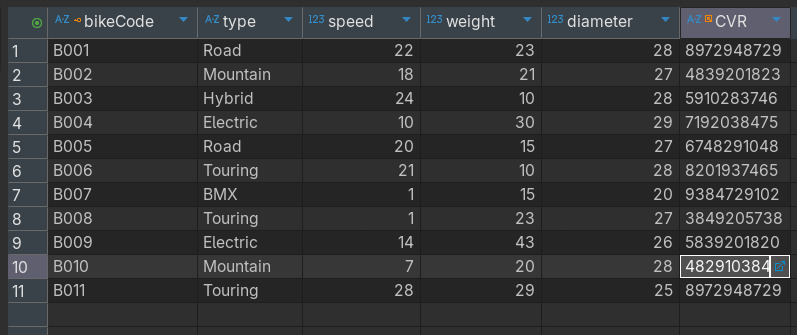
\includegraphics[width=0.9\linewidth]{figures/bikes_after_insert.png}
    \caption{Bikes table after inserting bicycle B011}
    \label{fig:bike-after}
\end{figure}

\subsubsection*{Multiple-Row Insertion}

The next example demonstrates inserting multiple rows at once into the \texttt{Compatibility} table.  
This corresponds to Figures~\ref{fig:compat-before} and \ref{fig:compat-after}.

\begin{lstlisting}[style=sql, caption={Insert multiple rows into the Compatibility table}, label={lst:insert-compat}]
INSERT INTO Compatibility (bikeCode, partCode)
VALUES
    ('B011', 'P009'),
    ('B001', 'P003'),
    ('B005', 'P002');
\end{lstlisting}


\begin{figure}[H]
    \centering
    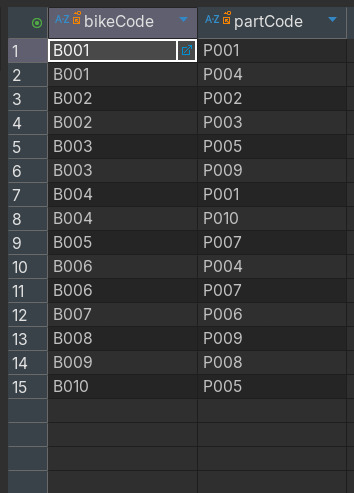
\includegraphics[width=0.45\linewidth]{figures/compat_before_insert.png}
    \caption{Compatibility table before multiple-row insertion}
    \label{fig:compat-before}
\end{figure}

\begin{figure}[H]
    \centering
    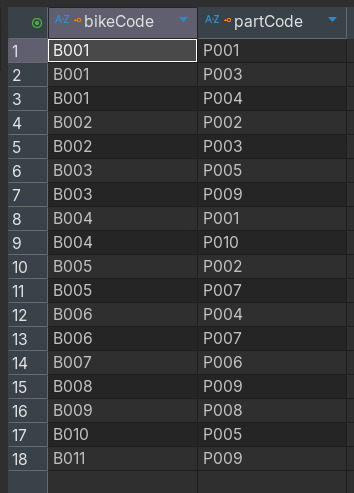
\includegraphics[width=0.45\linewidth]{figures/compat_after_insert.png}
    \caption{Compatibility table after multiple-row insertion}
    \label{fig:compat-after}
\end{figure}

\subsection{UPDATE Examples}

\subsubsection*{Updating Address When a Customer Moves House}

This example shows how an existing address is modified for a customer who moved.  
In the screenshots provided, the updated row corresponds to \texttt{CPR = '120385-5678'}.

\begin{lstlisting}[style=sql, caption={Update a customer's address after relocation}, label={lst:update-address}]
UPDATE Address
SET street = 'Tranevej',
    civicNumber = '18',
    zipCode = '8000'
WHERE CPR = '120385-5678';
\end{lstlisting}


\begin{figure}[H]
    \centering
    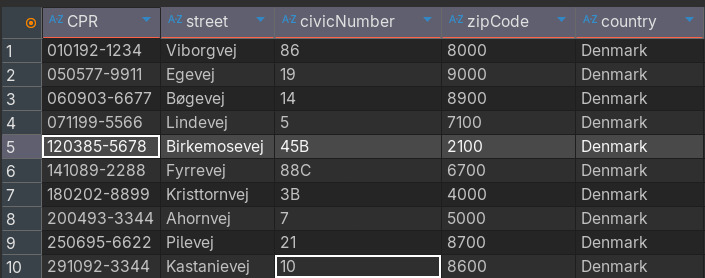
\includegraphics[width=0.9\linewidth]{figures/address_before_update.png}
    \caption{Address table before customer relocation update}
    \label{fig:address-before}
\end{figure}

\begin{figure}[H]
    \centering
    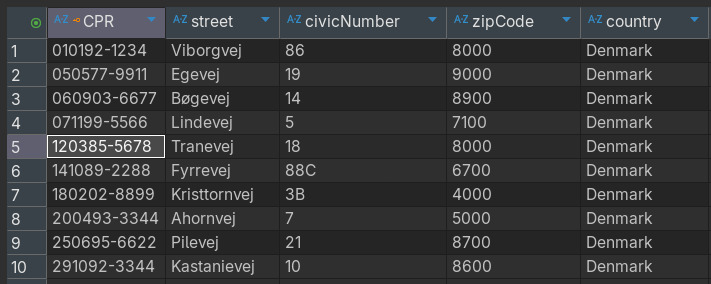
\includegraphics[width=0.9\linewidth]{figures/address_after_update.png}
    \caption{Address table after updating address for CPR 120385-5678}
    \label{fig:address-after}
\end{figure}

\subsection{DELETE Examples}

\subsubsection*{Removing a Customer's Phone Number}

The provided screenshots show deletion of the phone number \texttt{+4510101112}.  

\begin{lstlisting}[style=sql, caption={Delete a customer's phone number}, label={lst:delete-phone}]
DELETE FROM PhoneNumber
WHERE phoneNumber = '+4510101112';
\end{lstlisting}


\begin{figure}[H]
    \centering
    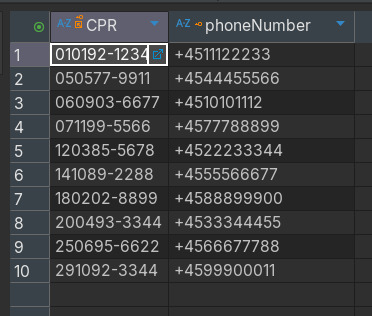
\includegraphics[width=0.5\linewidth]{figures/phone_before_delete.png}
    \caption{PhoneNumber table before deleting +4510101112}
    \label{fig:phone-before}
\end{figure}

\begin{figure}[H]
    \centering
    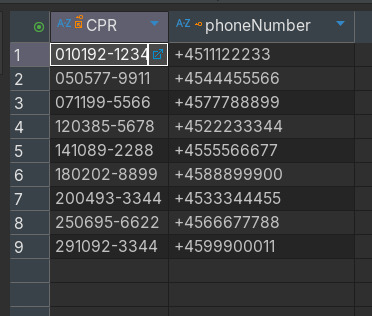
\includegraphics[width=0.5\linewidth]{figures/phone_after_delete.png}
    \caption{PhoneNumber table after deleting +4510101112}
    \label{fig:phone-after}
\end{figure}

\subsubsection*{Deleting a Discontinued Part}

In this example, a part is removed from the \texttt{Compatibility} table because it has been discontinued.  
The screenshot corresponds to deletion of \texttt{P002}.

\begin{lstlisting}[style=sql, caption={Delete a discontinued part from the Compatibility table}, label={lst:delete-part}]
DELETE FROM Compatibility
WHERE partCode = 'P002';
\end{lstlisting}

\begin{figure}[H]
    \centering
    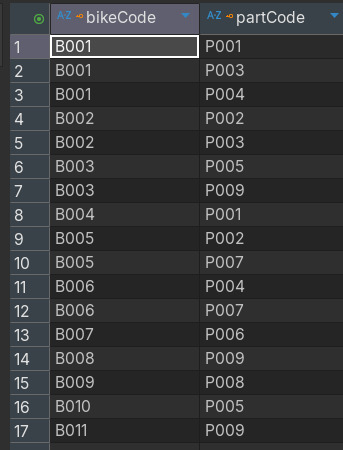
\includegraphics[width=0.45\linewidth]{figures/compat_before_delete.png}
    \caption{Compatibility table before deletion of part P002}
    \label{fig:part-before}
\end{figure}

\begin{figure}[H]
    \centering
    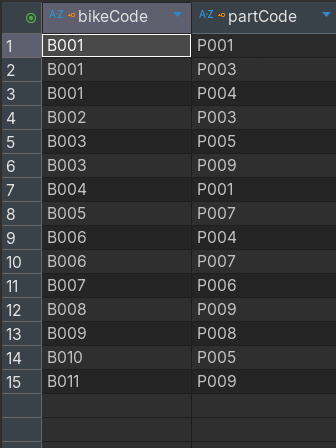
\includegraphics[width=0.45\linewidth]{figures/compat_after_delete.png}
    \caption{Compatibility table after deletion of part P002}
    \label{fig:part-after}
\end{figure}

% ========================================================

\section{SQL Data Queries}
% ========================================================

In this section, we present the five required SQL queries, each accompanied by:  
(1) the SQL code,  
(2) an informal explanation of the logic, and  
(3) the resulting output table, included as a figure.

All queries operate on the \texttt{DB} MariaDB schema.

% --------------------------------------------------------
\subsection{Query 1: Customers With a Bike Repaired More Than Once}
% --------------------------------------------------------

\begin{lstlisting}[style=sql, caption={Query to find customers with repeated repairs on the same bike}, label={lst:query1}]
USE DB;

SELECT DISTINCT CPR 
FROM RepairJob
GROUP BY CPR, bikeCode
HAVING COUNT(*) > 1;
\end{lstlisting}

To identify customers who have repaired the same bike more than once, we group by both \texttt{CPR} and \texttt{bikeCode}. This grouping ensures that repairs are counted per specific bike per customer. We then apply a \texttt{HAVING} clause to filter groups with more than one repair. Finally, \texttt{DISTINCT} is used to avoid duplicate CPRs in the output.

\begin{figure}[H]
    \centering
    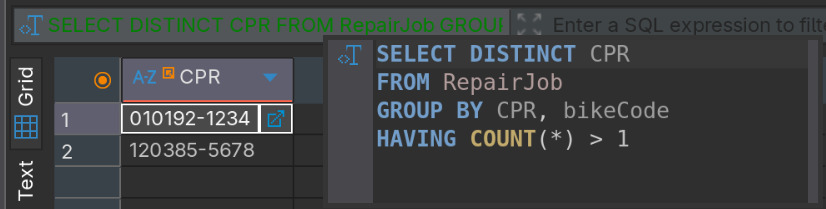
\includegraphics[width=0.65\linewidth]{figures/query1_results.png}
    \caption{Output of Query 1: Customers who repaired the same bike more than once.}
    \label{fig:query1}
\end{figure}


% --------------------------------------------------------
\subsection{Query 2: Parts Never Used in Any Repair}
% --------------------------------------------------------

\begin{lstlisting}[style=sql, caption={Query to find unused parts}, label={lst:query2}]
SELECT p.partCode, p.CVR
FROM RepairParts r RIGHT JOIN Parts p 
    ON r.partCode = p.partCode
WHERE quantity IS NULL;
\end{lstlisting}

This query identifies all parts that were never used in any repair.  
We perform a \texttt{RIGHT JOIN} from \texttt{RepairParts} to \texttt{Parts} so that all parts remain in the result, even if they have no matching repair record. When a part has never been used, its \texttt{quantity} field is \texttt{NULL} in the joined table, making it easy to filter.

\begin{figure}[H]
    \centering
    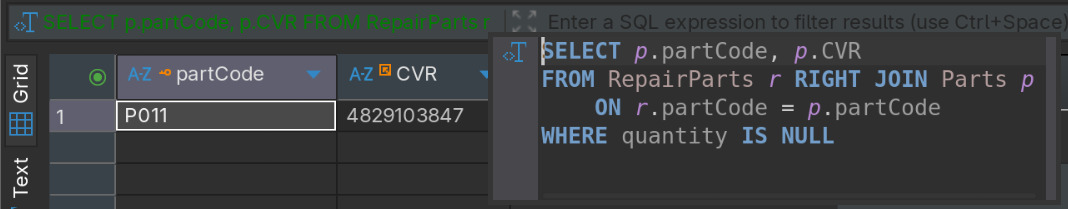
\includegraphics[width=0.65\linewidth]{figures/query2_results.png}
    \caption{Output of Query 2: Parts that were never used in any repair.}
    \label{fig:query2}
\end{figure}


% --------------------------------------------------------
\subsection{Query 3: Total Quantity Used per Part in 2024}
% --------------------------------------------------------

\begin{lstlisting}[style=sql, caption={Query to compute part usage in 2024}, label={lst:query3}]
SELECT r.partCode, p.CVR, SUM(r.quantity) AS 'Total quantity used'
FROM RepairParts r JOIN Parts p
    ON r.partCode = p.partCode
WHERE r.startDate >= '2024-01-01' AND r.startDate <= '2024-12-31'
GROUP BY r.partCode, p.CVR;
\end{lstlisting}

We compute the total usage of each part during the year 2024.  
The \texttt{WHERE} clause ensures that only repairs that \emph{start} in 2024 are included; this aligns with the idea that parts consumed in a repair are tied to its start date.  
After filtering, we group by \texttt{partCode} and \texttt{CVR} and compute the total quantity using \texttt{SUM()}.

\begin{figure}[H]
    \centering
    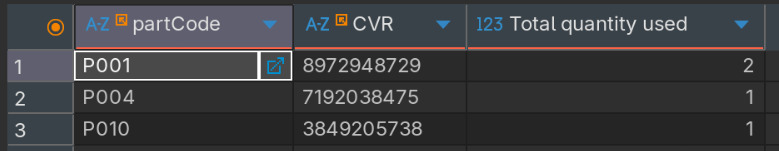
\includegraphics[width=0.65\linewidth]{figures/query3_results.png}
    \caption{Output of Query 3: Total quantity of each part used during 2024.}
    \label{fig:query3}
\end{figure}


% --------------------------------------------------------
\subsection{Query 4: Most Repaired Bike per Type}
% --------------------------------------------------------

\begin{lstlisting}[style=sql, caption={Views used to compute the most repaired bike per type}, label={lst:query4_views}]
CREATE VIEW mostRepairedBike AS (
    SELECT bikeCode, COUNT(*) AS tot
    FROM RepairJob
    GROUP BY bikeCode
);

CREATE VIEW mostRepairPerType AS (
    SELECT b.type, MAX(m.tot) AS maxTot
    FROM RepairJob r JOIN mostRepairedBike m 
        ON r.bikeCode = m.bikeCode 
        JOIN Bikes b 
        ON b.bikeCode = r.bikeCode
    GROUP BY b.type
);

CREATE VIEW rankBikes AS (
    SELECT b.type, b.bikeCode, b.CVR,
           ROW_NUMBER() OVER(
               PARTITION BY b.type 
               ORDER BY b.bikeCode ASC
           ) AS rnk
    FROM mostRepairedBike m JOIN Bikes b 
        ON m.bikeCode = b.bikeCode 
        JOIN mostRepairPerType mr
        ON mr.type = b.type
    WHERE m.tot = mr.maxTot
);
\end{lstlisting}

\begin{lstlisting}[style=sql, caption={Final query: Most repaired bike per type}, label={lst:query4}]
SELECT type, bikeCode, CVR
FROM rankBikes
WHERE rnk <= 1
ORDER BY type ASC;
\end{lstlisting}

This task requires identifying the most repaired bike within each bike type.  
We solve this in multiple steps:

1. \texttt{mostRepairedBike} view: Counts total repairs per bike.  
2. \texttt{mostRepairPerType} view: For each type, finds the maximum number of repairs.  
3. \texttt{rankBikes} view: Joins information and ranks tied bikes using \texttt{ROW\_NUMBER()}, partitioned by type.

The final query selects bikes with rank 1, yielding the most repaired bike(s) for each type.

\begin{figure}[H]
    \centering
    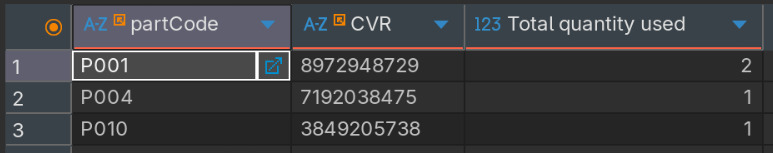
\includegraphics[width=0.75\linewidth]{figures/query4_results.png}
    \caption{Output of Query 4: Most repaired bike per bike type.}
    \label{fig:query4}
\end{figure}


% --------------------------------------------------------
\subsection{Query 5: Bikes Compatible Only With Parts From Their Own Manufacturer}
% --------------------------------------------------------

\begin{lstlisting}[style=sql, caption={Query to find bikes that can use only same-manufacturer parts}, label={lst:query5}]
SELECT DISTINCT b.bikeCode, b.CVR
FROM Compatibility c 
JOIN Bikes b ON c.bikeCode = b.bikeCode 
JOIN Parts p ON c.partCode = p.partCode
GROUP BY b.bikeCode, b.CVR
HAVING COUNT(DISTINCT p.CVR) = 1 
   AND b.CVR = MIN(p.CVR);
\end{lstlisting}

This query identifies bikes that are compatible exclusively with parts from the same manufacturer.  
We join \texttt{Bikes}, \texttt{Compatibility}, and \texttt{Parts}.  
If all compatible parts share the same manufacturer (\texttt{COUNT(DISTINCT p.CVR) = 1}) and that manufacturer equals the bike’s manufacturer (\texttt{b.CVR = MIN(p.CVR)}), then the bike meets the condition.

\begin{figure}[H]
    \centering
    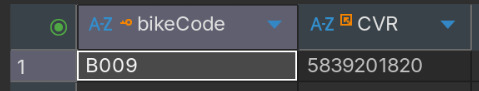
\includegraphics[width=0.65\linewidth]{figures/query5_results.png}
    \caption{Output of Query 5: Bikes using parts exclusively from their own manufacturer.}
    \label{fig:query5}
\end{figure}


%========================================================
\section{SQL Programming}
% ========================================================

In this section, we implement one function, one procedure, and several triggers in MariaDB in order to enforce data consistency and automate repair-related logic in the database. Each subsection provides the SQL code, an explanation of its purpose and internal logic, and an example of its usage through figures.

% --------------------------------------------------------
\subsection{Function: \texttt{getRepairPartsCost}}
% --------------------------------------------------------

\begin{lstlisting}[style=sql, caption={Definition of the getRepairPartsCost() function}, label={lst:getRepairPartsCost}]
DELIMITER //

CREATE FUNCTION getRepairPartsCost(
    CPR VARCHAR(11),
    bikeCode VARCHAR(10),
    startDate DATE,
    endDate DATE
)
RETURNS DECIMAL(10,2)
DETERMINISTIC
BEGIN
    DECLARE total DECIMAL(10,2);

    SELECT SUM(p.unitPrice * rp.quantity)
    INTO total
    FROM RepairParts AS rp
    JOIN Parts AS p ON rp.partCode = p.partCode
    WHERE rp.CPR = CPR
      AND rp.bikeCode = bikeCode
      AND rp.startDate = startDate
      AND rp.endDate = endDate;

    IF total IS NULL THEN
        SET total = 0;
    END IF;

    RETURN total;
END //

DELIMITER ;

SELECT getRepairPartsCost('050577-9911', 'B005', '2025-04-02', '2025-04-06') AS total_cost;
\end{lstlisting}

The \texttt{getRepairPartsCost()} function calculates the total price of all parts used in a specific repair job, identified by the arguments \texttt{CPR}, \texttt{bikeCode}, \texttt{startDate}, and \texttt{endDate}. Internally, the function defines a return type of \texttt{DECIMAL(10,2)}, allowing values up to \texttt{99,999,999.99}, and allocates a variable of the same type to store the computed result.


The core of the function is a \texttt{SELECT} statement that aggregates the total part cost using \texttt{SUM(unitPrice * quantity)}, performed through a join between the \texttt{Parts} and \texttt{RepairParts} tables. If the query finds no matching rows for the specified repair job, the function explicitly returns \texttt{0} instead of \texttt{NULL}, ensuring predictable behavior. The function is invoked using a standard \texttt{SELECT} statement, where all four identification arguments must be supplied.

\begin{figure}[H]
    \centering
    
\includegraphics[width=0.75\linewidth]{figures/getRepairPartsCost_proc.png}
    \caption{Example usage of \texttt{getRepairPartsCost()} when calculating part costs for a specific repair job.}
    \label{fig:getRepairPartsCostprocedure}
\end{figure}

\begin{figure}[H]
    \centering
    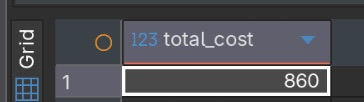
\includegraphics[width=0.75\linewidth]{figures/getRepairPartsCost_result.png}
    \caption{Generated cost using \texttt{getRepairPartsCost()}.}
    \label{fig:getRepairPartsCostresult}
\end{figure}


% --------------------------------------------------------
\subsection{Procedure: \texttt{addPartToRepair}}
% --------------------------------------------------------

\begin{lstlisting}[style=sql, caption={Definition of the addPartToRepair procedure}, label={lst:addPartToRepair}]
DELIMITER //

CREATE PROCEDURE addPartToRepair(
    IN inCPR VARCHAR(11),
    IN inBikeCode VARCHAR(10),
    IN inStartDate DATE,
    IN inEndDate DATE,
    IN inPartCode VARCHAR(10),
    IN inQuantity INT
)
BEGIN
    IF EXISTS (
        SELECT 1 FROM Compatibility
        WHERE bikeCode = inBikeCode AND partCode = inPartCode
    ) THEN
        INSERT INTO RepairParts (CPR, bikeCode, startDate, endDate, partCode, quantity)
        VALUES (inCPR, inBikeCode, inStartDate, inEndDate, inPartCode, inQuantity)
        ON DUPLICATE KEY UPDATE quantity = quantity + inQuantity;
    ELSE
        SIGNAL SQLSTATE '45000'
        SET MESSAGE_TEXT = 'This part is not compatible with this bike';
    END IF;
END //

DELIMITER ;

CALL addPartToRepair('050577-9911', 'B005', '2025-04-02', '2025-04-06', 'P007', 2);
\end{lstlisting}

The \texttt{addPartToRepair} procedure automates the insertion of parts into a repair job while ensuring compatibility and avoiding duplicate entries. All relevant identifiers (customer, bike, dates, part, and quantity) are passed in as arguments. The procedure begins by checking whether the specified part is compatible with the given bike using the \texttt{Compatibility} table.

If no compatible record is found, the procedure raises an error and aborts. Otherwise, the procedure inserts the part into the \texttt{RepairParts} table. When the same part is already associated with the repair job, the procedure automatically increases the quantity instead of inserting a new row, using an \texttt{ON DUPLICATE KEY UPDATE} clause. The procedure is executed via the \texttt{CALL} statement with all arguments specified.


\begin{figure}[H]
    \centering
    
\includegraphics[width=0.75\linewidth]{figures/addPartToRepair_result.png}
    \caption{Example usage of \texttt{addPartToRepair()} when adding a compatible part to a repair job.}
    \label{fig:addPartToRepair}
\end{figure}

\begin{figure}[H]
    \centering
    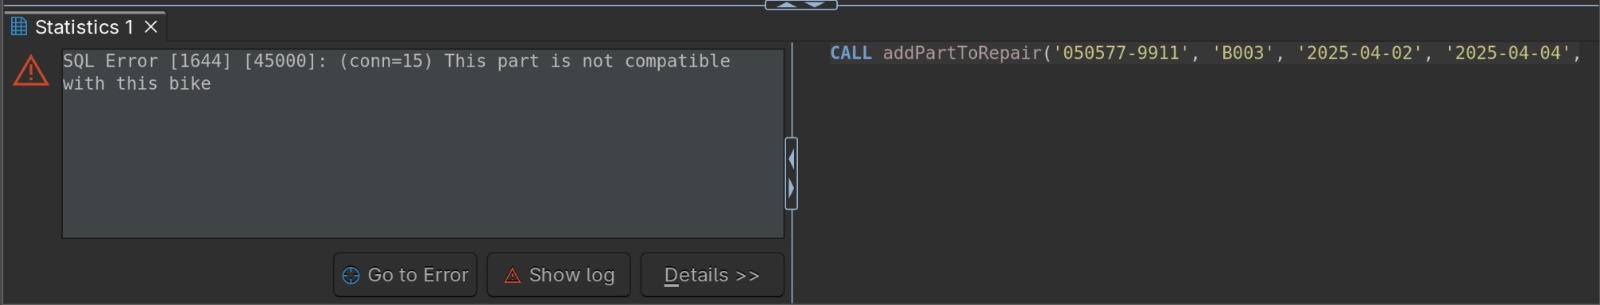
\includegraphics[width=0.75\linewidth]{figures/addPartToRepair_incorrect.png}
    \caption{Example usage of \texttt{addPartToRepair()} when adding an incompatible part and or bike to addPartsToRepair()}
    \label{fig:addPartToRepair}
\end{figure}


% --------------------------------------------------------
\subsection{Trigger: \texttt{checkRepairDuration}}
% --------------------------------------------------------

\begin{lstlisting}[style=sql, caption={Trigger to ensure repair duration does not exceed 3 days}, label={lst:checkRepairDuration}]
DELIMITER //

CREATE TRIGGER checkRepairDuration
BEFORE INSERT ON RepairJob
FOR EACH ROW
BEGIN
    DECLARE duration INT;

    SET duration = DATEDIFF(NEW.endDate, NEW.startDate);

    IF duration > 3 THEN
        SIGNAL SQLSTATE '45000'
        SET MESSAGE_TEXT = 'Repair cannot take longer than 3 days';
    END IF;
END //

DELIMITER ;
\end{lstlisting}

The \texttt{checkRepairDuration} trigger ensures that no repair job lasts longer than three days. Defined as a \texttt{BEFORE INSERT} trigger, it validates incoming data prior to insertion into the \texttt{RepairJob} table. The trigger computes the duration using \texttt{DATEDIFF(NEW.endDate, NEW.startDate)}, and if the result exceeds three days, it raises an error and prevents the insertion.

\begin{figure}[H]
    \centering
    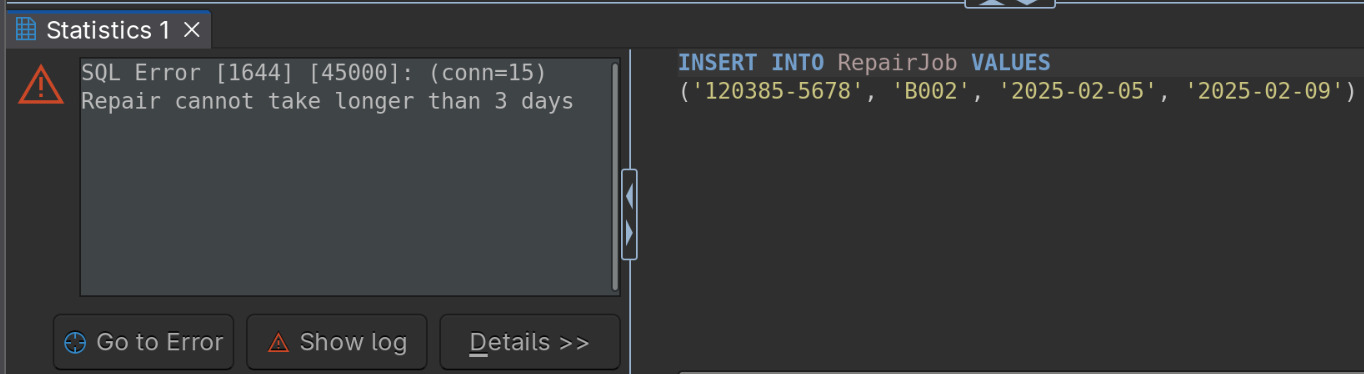
\includegraphics[width=0.75\linewidth]{figures/checkRepairDuration_result.png}
    \caption{Example of the \texttt{checkRepairDuration} trigger preventing an overly long repair job from being inserted.}
    \label{fig:checkRepairDuration}
\end{figure}


% --------------------------------------------------------
\subsection{Trigger: \texttt{checkRepairCost}}
% --------------------------------------------------------

\begin{lstlisting}[style=sql, caption={Trigger to ensure repair cost does not exceed 100,000 DKK}, label={lst:checkRepairCost}]
DELIMITER //

CREATE TRIGGER checkRepairCost
BEFORE INSERT ON RepairParts
FOR EACH ROW
BEGIN
    DECLARE totalCost DECIMAL(10,2);
    DECLARE newCost DECIMAL(10, 2);

    SET totalCost = getRepairPartsCost(
        NEW.CPR,
        NEW.bikeCode,
        NEW.startDate,
        NEW.endDate
    );

    SET newCost = (SELECT unitPrice 
                   FROM Parts 
                   WHERE partCode = NEW.partCode) 
                   * NEW.quantity;

    SET totalCost = totalCost + newCost;

    IF totalCost > 100000 THEN
        SIGNAL SQLSTATE '45000'
        SET MESSAGE_TEXT = 'Repair cost cannot be more than 100.000 dkk';
    END IF;
END //

DELIMITER ;
\end{lstlisting}

The \texttt{checkRepairCost} trigger prevents repair jobs from exceeding a total cost of 100,000 DKK. As a \texttt{BEFORE INSERT} trigger on the \texttt{RepairParts} table, it first retrieves the current total cost of the repair job via the previously defined \texttt{getRepairPartsCost()} function. It then computes the cost of the new part being inserted by multiplying its unit price by the specified quantity.

After adding the new part’s cost to the existing total, the trigger checks whether the updated amount surpasses the 100,000 DKK limit. If so, it raises an error and blocks the insertion, ensuring that repair jobs remain within the intended financial constraints.

\begin{figure}[H]
    \centering
    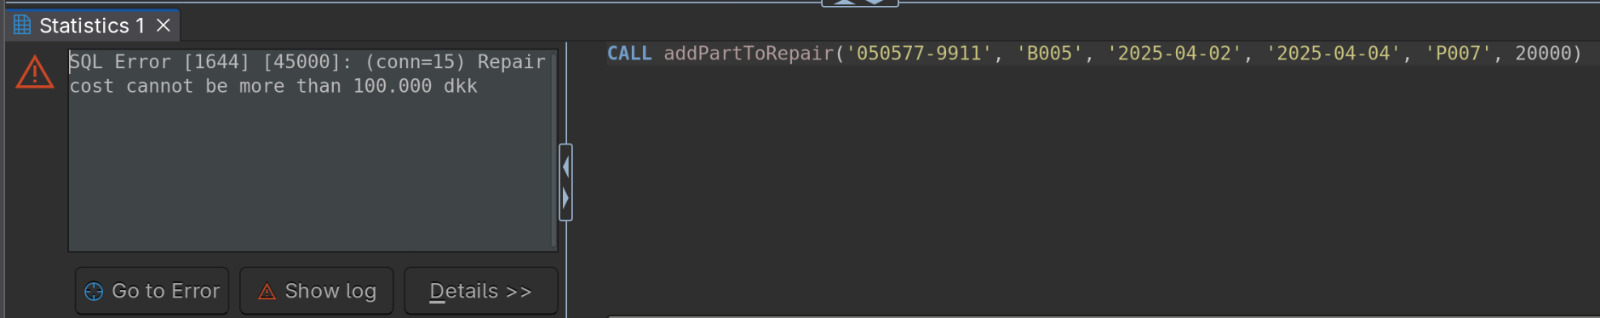
\includegraphics[width=0.75\linewidth]{figures/checkRepairCost_result.png}
    \caption{Example of the \texttt{checkRepairCost} trigger blocking an overly expensive repair.}
    \label{fig:checkRepairCost}
\end{figure}


% --------------------------------------------------------
\subsection{Trigger: \texttt{checkCPR} (Extra)}
% --------------------------------------------------------

\begin{lstlisting}[style=sql, caption={Trigger to validate CPR format}, label={lst:checkCPR}]
DELIMITER //

CREATE TRIGGER checkCPR
BEFORE INSERT ON Customer
FOR EACH ROW
BEGIN 
  IF NEW.CPR NOT REGEXP '^[0-9]{6}-[0-9]{4}$' THEN 
    SIGNAL SQLSTATE '45000'
    	SET MESSAGE_TEXT = 'Invalid CPR Number';
  END IF;
END//

DELIMITER ;
\end{lstlisting}

The \texttt{checkCPR} trigger enforces a consistent structural format for customer CPR numbers, requiring the pattern \texttt{XXXXXX-XXXX}. Activated \texttt{BEFORE INSERT}, the trigger validates the input using a regular expression: six digits, a hyphen, and four digits, with the \texttt{\^} and \texttt{\$} anchors ensuring that the entire string adheres strictly to this pattern. Although real Danish CPR numbers encode a valid date in the first six digits, this trigger validates only the structural format, not the semantic correctness.

\begin{figure}[H]
    \centering
    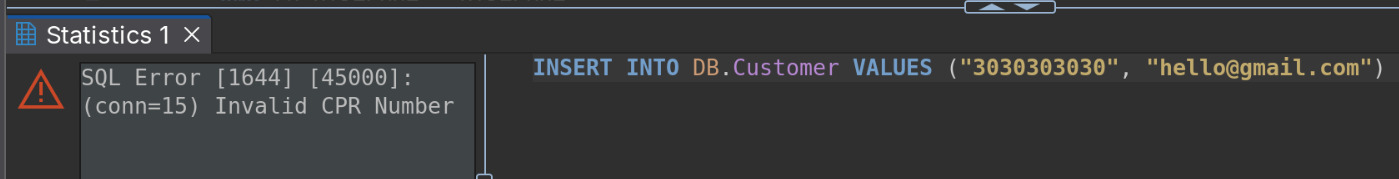
\includegraphics[width=0.75\linewidth]{figures/checkCPR_result.png}
    \caption{Example usage of the \texttt{checkCPR} trigger rejecting an incorrectly formatted CPR number.}
    \label{fig:checkCPR}
\end{figure}


% ========================================================
\section*{Closing Discussion}

In this project, we successfully designed and implemented a comprehensive relational database for Cykelparadis. The conceptual model captured all essential entities and relationships, and the logical design translated these into normalized tables that prevent redundancy and maintain data integrity. We ensured accuracy and flexibility through key design decisions, such as: using CVR numbers as primary keys for manufacturers, decomposing addresses into separate tables, and implementing many-to-many relationships via bridge tables.

The SQL implementation demonstrated core data manipulation operations (\texttt{INSERT}, \texttt{UPDATE}, \texttt{DELETE}) as well as advanced querying capabilities, including aggregation, filtering, and joins. Programming constructs-functions, procedures, and triggers; were employed to automate calculations, enforce business rules, and maintain data consistency.

Overall, the project illustrates how careful database design, coupled with precise SQL programming, can support complex operations and maintain data reliability in a practical business scenario. Future improvements could include further automation of repair scheduling, enhanced reporting for parts usage and cost tracking, and extending the database to support additional services or sales analytics. The workflow of this project reinforces the importance of combining theoretical database principles with practical implementation to achieve a robust and maintainable system.

% ========================================================
\section*{Use of GenAI}
Generative AI tools (\textit{ChatGPT} by OpenAI and \textit{Claude} by Anthropic) were used only for assistance with syntax checking and \LaTeX{} formatting.

All conceptual, logical, and implementation decisions were made by the project group members based on the actual SQL execution results and the official course material.

\bibliography{citations}
\bibliographystyle{unsrt}

\vspace*{1cm}
\appendix
\LARGE\bfseries Appendix
\normalsize\normalfont

% ========================================================
\section{Supplementary Material}
% ========================================================

\subsection{Project GitHub Repository}

All project files are available in our GitHub repository for reference and reproducibility.  
The repository contains all scripts, the final PDF report, and the effort tracking spreadsheet used by our group.

\textbf{Repository Link:} \url{https://github.com/DiegoA-ML/Cykelparadis-DatabaseCreation/tree/main}

\subsubsection*{Contents of the Repository}

The repository includes the following files:

\begin{itemize}
    \item \texttt{08\_02327GroupReport2025.pdf} ; This final group project report containing all sections: conceptual design, logical design, implementation, SQL modifications, queries, and programming.
    \item \texttt{08\_02327DatabaseScript1\_2025.sql} ; SQL script for creating the database, its tables, and views; also includes population of the tables.
    \item \texttt{08\_02327DatabaseScript2\_2025.sql} ; SQL script for table modifications (INSERT, UPDATE, DELETE), all queries, and SQL programming elements (triggers, functions, procedures).
    \item \texttt{08\_02327Effort\_2025.xlsx} ; Spreadsheet documenting individual contributions of each group member for every task.
\end{itemize}

These materials ensure that the database, queries, and project results are fully reproducible and can be easily inspected for correctness and completeness.

\end{document}
